\documentclass[journal]{IEEEtran}
\usepackage{fontspec}
\usepackage{unicode-math}
\setmainfont{TeX Gyre Termes}
\setmathfont{Latin Modern Math}
\setmonofont{Latin Modern Mono}
\usepackage{graphicx}
\usepackage{booktabs,tabularx,array}
\usepackage{enumitem}
\setlist{itemsep=2pt,topsep=4pt,parsep=0pt}
\usepackage{listings}
\lstset{basicstyle=\ttfamily\small,columns=fullflexible,keepspaces=true,mathescape=true,breaklines=true,frame=lines,framesep=4pt,aboveskip=8pt,belowskip=8pt}
\usepackage[hyphens]{url}
\usepackage[hidelinks]{hyperref}
\usepackage{caption}
\captionsetup{font=small,labelfont=bf,labelsep=period}
\providecommand{\mdlgwhtsquare}{$\square$}
\providecommand{\tightlist}{\setlength{\itemsep}{2pt}\setlength{\parskip}{0pt}}
\renewcommand{\arraystretch}{1.15}
\begin{document}
\title{Confluent Accumulation Cells: Bounded-State, Order-Invariant Floating-Point Scatter-Add}
\author{\IEEEauthorblockN{Aditya Raj\thanks{Research status: the evidence in this paper comes from a software reference model of a GPU and from CPU threads. Validation on physical GPUs remains future work.}}
\IEEEauthorblockA{School of Artificial Intelligence and Data Science\\Indian Institute of Technology Jodhpur, Jodhpur, India}}
\maketitle
\begin{abstract}
Floating-point scatter-add on a GPU returns different bits from run to run. Atomic operations guarantee that every update is applied, but not the order, and floating-point addition is not associative. Existing remedies sort the contributions, assume the value range in advance, read the data twice, or keep an exact accumulator of hundreds to thousands of bits per destination. We present Confluent Accumulation Cells (CAC). Each destination holds K 64-bit cells, with K between 2 and 4. A cell stores an 8-bit bin tag and a 56-bit integer, and two cells combine by the rule ``the larger tag wins, equal tags add''. This operation forms a commutative monoid, so the final state cannot depend on commit order, warp-level combining or multi-device merging. CAC reads each contribution once and needs no prior knowledge of the value range. Its error is below n × \(2^{-(K-1)W}\) times the largest addend, and it is zero when the dynamic range of the addends fits the window. We evaluate CAC in a virtual-GPU reference model against eight baselines and an exact big-integer oracle. Plain atomic addition produced 32 different output vectors under 32 schedules in all 28 combinations of format and test case. CAC produced one output in every case and passed all 420 invariance checks. For binary64 data, CAC with 24 bytes per destination matched the correctly rounded sum on all but one of 53,248 destinations in 13 of 14 cases; the exact superaccumulator in our model needs 532 bytes. The fourteenth case, cancellation of near-overflow pairs, defeats CAC: it returns zero where the true result is of order one. Two further results limit the claim. For binary32 data, accumulating in binary64 was as accurate as CAC on 13 of 14 cases, so there CAC adds a guarantee and not accuracy. All evidence comes from the simulator, and we make no physical-GPU timing claim.
\end{abstract}
\begin{IEEEkeywords}
floating-point reproducibility, GPU atomic operations, order invariance, scatter-add
\end{IEEEkeywords}
\hypertarget{introduction}{%
\section{Introduction}\label{introduction}}

Scatter-add writes many contributions into few destinations: y{[}d{]} +=
x for a stream of pairs (d, x). It is the core of histograms, index\_add
and scatter\_add, embedding-gradient accumulation, the backward pass of
gather and interpolation, particle-to-grid deposition, splatting and
force accumulation. On a GPU the usual implementation is one atomicAdd
per contribution.

An atomic add is safe but not ordered. It guarantees that no update is
lost; it does not fix the order in which updates reach a destination.
Floating-point addition is not associative {[}1, 2{]}, so each order can
round differently and the same program returns different bits on
different runs.

The effect is documented and unresolved in practice. Shanmugavelu et
al.~measure the run-to-run variability of atomic kernels and the cost of
replacing them with deterministic alternatives {[}3{]}. The PyTorch
documentation lists CUDA operations, among them index\_add\_, histc,
weighted bincount and the backward passes of grid\_sample and several
interpolation modes, that either switch to a slower deterministic
implementation or raise an error under
torch.use\_deterministic\_algorithms(True) {[}4{]}. Cankaya finds GPU
inference bit-reproducible on identical hardware and reproduces it
across GPU types with an emulator; floating-point atomics were the only
true source of run-to-run variation in those experiments {[}5{]}.

Bit-level reproducibility matters for regression testing, for debugging,
for auditing a computation by re-running it, and for getting the same
answer from one GPU and from eight. A result that changes with the
thread schedule can satisfy none of these.

Existing remedies each give up something. Deterministic hardware and
schedulers fix one order, at an architectural cost {[}6, 7{]}.
Sort-based reductions need scratch memory proportional to the input and
depend on the input order. Fixed-point accumulation needs the value
range in advance {[}8{]}. A two-pass window reads every contribution
twice. Exact superaccumulators are invariant and correct but need
hundreds to thousands of bits per destination {[}9, 10{]}.

This paper asks whether a small, fixed number of words per destination
can give order invariance in one pass with no range assumption.
Confluent Accumulation Cells do so by making each word a commutative
monoid: the exponent window and the digit live in the same 64-bit word,
so choosing the window and adding into it is one atomic step.

\hypertarget{research-questions}{%
\subsection{Research questions}\label{research-questions}}

\begin{enumerate}
\def\labelenumi{\arabic{enumi}.}
\item
  \textbf{RQ1.} Can the irreproducibility of floating-point scatter-add
  be reproduced deterministically, from a seed, in a model of GPU
  execution?
\item
  \textbf{RQ2.} Is there a bounded-state, single-pass mechanism whose
  output is a function of the multiset of contributions alone?
\item
  \textbf{RQ3.} How accurate is it, and where does it fail?
\item
  \textbf{RQ4.} What does it cost in state and atomic operations against
  the known alternatives?
\end{enumerate}

\hypertarget{contributions}{%
\subsection{Contributions}\label{contributions}}

\begin{itemize}
\item
  \textbf{A reproducible problem.} A seeded 14-case workload matrix and
  five scheduler families make every schedule-dependent result
  repeatable.
\item
  \textbf{A mechanism.} CAC uses K max-tagged 64-bit cells per
  destination on an absolute grid of W-bit bins (Section 4).
\item
  \textbf{Proofs.} The cell operation is a commutative monoid, the final
  state is confluent, and the error is bounded relative to the largest
  addend (Section 5).
\item
  \textbf{A working model.} A C++17 virtual GPU with eight baselines, an
  exact oracle, 55 tests and an independent Python cross-check (Section
  6).
\item
  \textbf{An evaluation that includes the failures.} One case defeats
  CAC, binary64 needs K $\geq$ 3, and binary64 accumulation is a strong
  baseline for binary32 data (Sections 8 to 10).
\end{itemize}

\hypertarget{claim-boundary}{%
\subsection{Claim boundary}\label{claim-boundary}}

Every number in this paper comes from the reference simulator. The
simulator establishes functional behaviour: which bits come out, under
which schedules, with how many atomic operations. It does not establish
the speed of CAC on a physical GPU, and no CUDA kernel was run.

\hypertarget{the-reproducible-problem}{%
\section{The reproducible problem}\label{the-reproducible-problem}}

\hypertarget{setting}{%
\subsection{Setting}\label{setting}}

A scatter-add has D destinations with initial values and n contributions
(d, x). The intended result at destination d is the initial value plus
the sum of every x sent to d.~A GPU kernel runs one lane per
contribution, and each lane issues atomicAdd(\&y{[}d{]}, x).

Any interleaving of those atomic operations is a legal execution. The
hardware scheduler, the launch configuration, the driver version and the
number of devices all change the interleaving, and none of them is under
the program's control.

\hypertarget{three-witnesses}{%
\subsection{Three witnesses}\label{three-witnesses}}

Three small multisets show that both the value and the IEEE class of the
result depend on order. All are binary32; M is the largest finite value,
about \(3.4\times10^{38}\).

\begin{table}[!htbp]\centering\small\setlength{\tabcolsep}{4pt}
\caption{Order dependence of the value and IEEE class for three binary32 multisets.}\label{tab:1}
\begin{tabularx}{\linewidth}{>{\raggedright\arraybackslash\hsize=0.588\hsize}X>{\raggedright\arraybackslash\hsize=1.373\hsize}X>{\raggedright\arraybackslash\hsize=1.490\hsize}X>{\raggedright\arraybackslash\hsize=0.549\hsize}X}
\toprule
Addends at one destination & One legal order gives & Another legal order gives & Exact sum, correctly rounded \\
\midrule
\(2^{24}\), 1, 1 & 16,777,216 (each 1 is rounded away) & 16,777,218 (1 + 1 first) & 16,777,218 \\
M, M, −M & +Inf (M + M overflows first) & M (M − M first) & M \\
M, M, −M, −M & +Inf or −Inf & 0, or NaN when two devices merge +Inf and −Inf & 0 \\
\bottomrule
\end{tabularx}
\end{table}

The first witness is ordinary rounding. The second and third are worse:
an intermediate overflow turns a finite sum into an infinity or a NaN,
and the class of the output depends on the schedule.

\hypertarget{problem-statement}{%
\subsection{Problem statement}\label{problem-statement}}

Find a per-destination state, a deposit rule, a merge rule and a
read-out such that the output is a function of the multiset of
contributions only. We require five properties.

\begin{table}[!htbp]\centering\small\setlength{\tabcolsep}{4pt}
\caption{Requirements R1 to R5 for an order-invariant scatter-add.}\label{tab:2}
\begin{tabularx}{\linewidth}{>{\raggedright\arraybackslash\hsize=0.733\hsize}X>{\raggedright\arraybackslash\hsize=1.267\hsize}X}
\toprule
Requirement & Meaning \\
\midrule
R1 Order invariance & Identical bits under any legal schedule, any permutation of the
contributions, any split across devices followed by a merge, and any
pre-combination inside a warp \\
R2 Bounded state & A fixed number of words per destination, independent of n and of the
value range \\
R3 Single pass & Each contribution is read once; no sort and no scratch memory
proportional to n \\
R4 No range assumption & Correct handling of any finite value, subnormals, signed zeros,
infinities and NaN, with nothing known in advance \\
R5 Stated accuracy & A proven bound on the distance to the exact sum \\
\bottomrule
\end{tabularx}
\end{table}

R1 is stronger than run-to-run determinism. A scheme that fixes one
order is deterministic on one device with one input order, and still
changes its answer when the batch is shuffled or split across devices.

\hypertarget{a-problem-that-can-be-re-run}{%
\subsection{A problem that can be
re-run}\label{a-problem-that-can-be-re-run}}

On real hardware the irreproducibility is itself hard to reproduce,
because the schedule cannot be chosen. The reference model makes the
schedule an explicit, seeded input. The same seed always gives the same
interleaving, so each ``different run'' in this paper can be regenerated
exactly (Sections 6 and 7).

\hypertarget{related-work-and-the-gap}{%
\section{Related work and the gap}\label{related-work-and-the-gap}}

No approach we surveyed meets R1 to R5 together. Table \ref{tab:3}
places each family against the requirements; the paragraphs below give
the detail.

\begin{table}[!hb]\centering\footnotesize\setlength{\tabcolsep}{4pt}
\caption{Prior approaches against requirements R1 to R5.}\label{tab:3}
\begin{tabularx}{\linewidth}{>{\raggedright\arraybackslash\hsize=1.261\hsize}X>{\raggedright\arraybackslash\hsize=1.261\hsize}X>{\raggedright\arraybackslash\hsize=1.261\hsize}X>{\raggedright\arraybackslash\hsize=0.431\hsize}X>{\raggedright\arraybackslash\hsize=0.365\hsize}X>{\raggedright\arraybackslash\hsize=1.161\hsize}X>{\raggedright\arraybackslash\hsize=1.261\hsize}X}
\toprule
Approach & Representative work & State per destination & Passes & Range needed in advance & Invariant to schedule / permutation / device split & Accuracy \\
\midrule
Floating-point atomic add & status quo & 4 or 8 B & 1 & no & no / no / no & depends on order \\
Deterministic architecture or scheduling & GPUDet {[}6{]}, DAB {[}7{]} & 4 or 8 B & 1 & no & yes / not addressed / not addressed & that of one fixed order \\
Sort, then add in index order & deterministic fallbacks {[}3, 4{]} & scratch memory $\propto$ n & 1 plus a sort & no & yes / no / no & that of one fixed order \\
Fixed-point integer atomics & SPFP {[}8{]}, {[}18{]} & 8 B & 1 & \textbf{yes} & yes / yes / yes & exact inside the chosen window \\
Wider floating-point accumulator & common practice & 8 B, binary32 data only & 1 & no & not guaranteed & near exact for binary32 \\
Pre-rounding against a maximum found first & Demmel and Nguyen {[}11{]} & 2 words & \textbf{2} & no & yes / yes / yes & bounded \\
Exact long accumulator & {[}9, 10, 14, 15{]} & 280 bits (binary32), about 2,100 bits (binary64) {[}9{]} & 1 & no & yes / yes / yes & exact \\
Binned reproducible sum & ReproBLAS {[}12{]}, RDBMS aggregation {[}13{]} & 6 words by default & 1 & no & yes / yes / yes, for reductions & bounded \\
\textbf{Confluent Accumulation Cells} & this paper & 16 to 32 B & 1 & no & yes / yes / yes & bounded relative to the largest addend \\
\bottomrule
\end{tabularx}
\end{table}

\textbf{Deterministic execution.} GPUDet makes a whole GPU program
deterministic at roughly a twofold slowdown {[}6{]}. Deterministic
Atomic Buffering targets atomics alone and reports a 23\% slowdown
{[}7{]}. Both fix one order. They need hardware changes, and the result
still changes when the input order or the device count changes.

\textbf{Atomic addition specifically.} Defour and Collange study exactly
this operation {[}9{]}. They propose work reassignment, which enforces
an order, and fixed-point accumulation in a long accumulator updated
with integer atomics, which is exact. For the long accumulator they
report overheads of 1.3× to 21× over unordered atomic addition, and 0.4×
to 10× for work reassignment. Their accumulator is complete: it covers
the whole exponent range, which is what makes it large.

\textbf{Exact and reproducible summation.} Long accumulators go back to
Kulisch {[}15{]} and were made fast on multi-core and GPU reductions by
ExBLAS {[}10{]} and by Neal {[}14{]}. Demmel and Nguyen replace
exactness with pre-rounding into bins {[}11{]}; Ahrens, Demmel and
Nguyen turn this into a six-word binned accumulator {[}12{]}, and Müller
et al.~apply it to grouped sums in a database engine {[}13{]}. These
designs target reductions, where each thread owns a private accumulator.
When a larger value arrives, a binned accumulator shifts several words
together. To our knowledge none of them is formulated as a shared cell
that many lanes update lock-free.

\textbf{Practice.} GPU molecular dynamics accumulates forces in 64-bit
fixed point with a scale chosen in advance {[}8{]}. Users of a GPU
quantum-chemistry code have proposed fixed-point integer atomics to make
energies and gradients repeat bit for bit, and its maintainers have
raised the overflow risk of the fixed scale {[}18{]}, and an inference
runtime documents that its binary32 scatter-sum is not bit-reproducible
{[}19{]}. Each is a local workaround for the general problem.

\textbf{Replicated data types.} A state-based CRDT converges because its
merge is associative, commutative and idempotent {[}16{]}. CAC uses the
same algebraic route to order independence, with a commutative monoid in
place of a semilattice, since a sum must count every deposit once.

\hypertarget{novelty-boundary}{%
\subsection{Novelty boundary}\label{novelty-boundary}}

The ingredients of CAC are known: digits of a long accumulator, an
exponent window anchored at the largest addend, and integer atomics. We
claim the combination. The bin tag is stored in the same word as the
digit, so selecting the window and accumulating into it is a single
atomic operation of a commutative monoid. That removes the first pass of
a window scheme and the unused words of a superaccumulator. We found no
prior description of this construction in the work cited here, and we
limit the claim to that survey.

\hypertarget{confluent-accumulation-cells}{%
\section{Confluent Accumulation
Cells}\label{confluent-accumulation-cells}}

Notation. We write \(\mathcal{G}\) for the absolute grid of a format,
\(\mathcal{B}\) for the set of its bins, \(\mathcal{C}\) for the set of
cells, and \(\oplus\) for the cell operation. A cell is a pair
\(c=(t,v)\in\mathcal{C}\) with tag \(t\in\{0,\dots,255\}\) and value
\(v\in\mathbb{Z}_{2^{56}}\), and the empty cell is \(\mathbf{0}=(0,0)\).

CAC keeps, for each destination, the top K bins of an exact long
accumulator, and lets the bins that hold them be chosen by the data as
it arrives.

\hypertarget{the-absolute-grid}{%
\subsection{The absolute grid}\label{the-absolute-grid}}

Every finite value of a format is an integer multiple of its smallest
subnormal. A binary32 value is ±m × \(2^q\) grid units of \(2^{-149}\),
with m below \(2^{24}\); the whole format fits in 277 bits. A binary64
value uses units of \(2^{-1074}\) and fits in 2,098 bits. On this grid,
addition is integer addition and is exact.

\hypertarget{bins-and-digits}{%
\subsection{Bins and digits}\label{bins-and-digits}}

The grid is cut into bins of W bits; bin j covers bit positions jW to
(j+1)W − 1. A value is sliced into its base-\(2^W\) digits, one per bin
it touches. With W = 32, a binary32 value touches at most 2 bins and a
binary64 value at most 3. A negative value contributes negated digits.

An exact superaccumulator stores one word for every bin: 9 words for
binary32 and 66 for binary64 at W = 32. CAC stores K.

\hypertarget{the-max-tagged-bin-cell}{%
\subsection{The max-tagged-bin cell}\label{the-max-tagged-bin-cell}}

A cell is one 64-bit word: an 8-bit tag in the high byte and a 56-bit
two's-complement value. Tag 0 is the empty cell. Two cells combine as
follows.

\[(t_1,v_1)\oplus(t_2,v_2)=\begin{cases}(t_1,\,v_1+v_2 \bmod 2^{56}) & t_1=t_2\\(t_1,v_1) & t_1>t_2\\(t_2,v_2) & t_1<t_2\end{cases}\]

In words: the larger tag wins and discards the other cell; equal tags
add their values.

\hypertarget{slots}{%
\subsection{Slots}\label{slots}}

A destination owns K cells, called slots. A digit of bin j is deposited
into slot j mod K with tag j + 2. Bins that are K apart share a slot,
and the higher bin evicts the lower one. The K slots therefore converge
on the highest bins that received data, whatever order the data arrived
in.

\hypertarget{deposit}{%
\subsection{Deposit}\label{deposit}}

A lane decodes its value, slices it, and for each non-zero digit applies
the cell operation to one slot. On current GPUs this is a
compare-and-swap loop on a 64-bit word:

\begin{enumerate}
\def\labelenumi{\arabic{enumi}.}
\item
  Load the slot.
\item
  If the slot's tag is larger than the digit's tag, stop: the digit can
  never be retained (Lemma 2).
\item
  Compute the combined cell and attempt a compare-and-swap. On failure,
  take the returned word and go to step 2.
\end{enumerate}

A device with a native read-modify-write instruction for this operation
would issue step 3 alone, with no load and no retry. The model evaluates
both forms. The initial value of a destination is deposited like any
contribution.

\hypertarget{read-out}{%
\subsection{Read-out}\label{read-out}}

After the kernel, each destination is read once. The retained digits are
summed as an exact integer, each shifted to its bin position, and the
integer is rounded to the target format once, to nearest with ties to
even. If the rounded value exceeds the largest finite number, the result
is an infinity, as IEEE 754 prescribes for the exact sum {[}17{]}. No
intermediate overflow can occur.

\hypertarget{special-values}{%
\subsection{Special values}\label{special-values}}

Three reserved tags carry the non-finite cases without extra state.

\begin{table}[!htbp]\centering\small\setlength{\tabcolsep}{4pt}
\caption{Reserved tags for non-finite values.}\label{tab:4}
\begin{tabularx}{\linewidth}{>{\raggedright\arraybackslash\hsize=0.295\hsize}X>{\raggedright\arraybackslash\hsize=0.505\hsize}X>{\raggedright\arraybackslash\hsize=1.600\hsize}X>{\raggedright\arraybackslash\hsize=1.600\hsize}X}
\toprule
Tag & Class & Value field & Read-out \\
\midrule
1 & zero & count of +0 in the low 28 bits, of −0 in the high 28 & −0 only if every addend was −0; ignored when any finite digit is present \\
NB + 2 & infinity & count of +Inf low, −Inf high & +Inf or −Inf; NaN if both are present \\
NB + 3 & NaN & count & NaN \\
\bottomrule
\end{tabularx}
\end{table}

NB is the number of bins. The infinity and NaN tags exceed every finite
tag, so no finite deposit can evict them. The 8-bit tag requires NB + 3
$\leq$ 255, which holds for W $\geq$ 16 in both formats.

\hypertarget{a-worked-example}{%
\subsection{A worked example}\label{a-worked-example}}

Take the first witness of Section 2 with K = 2 and W = 32. The value 1
is bit 149 of the grid, in bin 4, with digit \(2^{21}\). The value
\(2^{24}\) is bit 173, in bin 5, with digit \(2^{13}\).

\begin{table}[!htbp]\centering\small
\caption{Cell states in the worked example ($K=2$, $W=32$).}\label{tab:5}
\begin{tabular}{lll}
\toprule
Deposit & Slot 0 (even bins) & Slot 1 (odd bins) \\
\midrule
\(2^{24}\) & empty & tag 7, value \(2^{13}\) \\
1 & tag 6, value \(2^{21}\) & tag 7, value \(2^{13}\) \\
1 & tag 6, value \(2^{22}\) & tag 7, value \(2^{13}\) \\
\bottomrule
\end{tabular}
\end{table}

The read-out is \(2^{13}\) × \(2^{160}\) + \(2^{22}\) × \(2^{128}\) grid
units, which is 16,777,218 exactly. Any other order of the three
deposits ends in the same two cells.

\hypertarget{analysis}{%
\section{Analysis}\label{analysis}}

Three results carry the design: the cell operation is a commutative
monoid, the final state is therefore independent of order, and the
discarded part is bounded.

\hypertarget{the-cell-monoid}{%
\subsection{The cell monoid}\label{the-cell-monoid}}

\textbf{Lemma 1 (canonical form).} Folding any finite sequence of cells
with $\oplus$, in any bracketing, gives the cell below, where t* is the largest
tag in the sequence.

\[\bigoplus_i (t_i,v_i)=\Bigl(t^*,\ \sum_{i:\,t_i=t^*} v_i \bmod 2^{56}\Bigr)\]

\emph{Proof.} By induction on the length. Combining a canonical cell
with one more cell either raises the tag and restarts the sum, keeps the
tag and extends the sum, or leaves the cell unchanged. Each outcome is
the canonical form of the longer sequence. \hfill$\mdlgwhtsquare$

\textbf{Theorem 1.} The set of cells \(\mathcal{C}\) with \(\oplus\) and
the empty cell \(\mathbf{0}\) forms a commutative monoid
\((\mathcal{C},\oplus,\mathbf{0})\).

\emph{Proof.} The definition is symmetric, so $\oplus$ commutes. The empty cell
has tag 0 and loses to every deposit. By Lemma 1, (a $\oplus$ b) $\oplus$ c and a $\oplus$ (b
$\oplus$ c) both equal the canonical form of \{a, b, c\}. \hfill$\mdlgwhtsquare$

\hypertarget{confluence}{%
\subsection{Confluence}\label{confluence}}

\textbf{Lemma 2 (drop rule).} The tag of a cell never decreases. If a
lane observes a cell whose tag exceeds the tag t of its digit, then c $\oplus$
(t, v) = c for every later state c of that cell. Skipping the deposit is
the same as applying it.

\textbf{Theorem 2 (order invariance).} Assume each cell update is atomic
and each deposit is applied once or skipped under Lemma 2. Then the
final state of every cell is the canonical form of the multiset of
deposits addressed to it. The output is identical under any schedule,
any permutation of the contributions, any combining of deposits inside a
warp, and any split across devices whose cells are merged with $\oplus$.

\emph{Proof.} Atomicity gives each cell a sequence of applied deposits.
By Lemma 2 the skipped ones can be appended without effect. By Lemma 1
the fold of the sequence depends only on its multiset. Warp combining
and device merging re-bracket the same fold, which Theorem 1 permits.
The read-out is a function of the cells. \hfill$\mdlgwhtsquare$

The theorem is about the final state. Intermediate states differ between
schedules, and CAC must not be read before the kernel has finished.

\hypertarget{error-bound}{%
\subsection{Error bound}\label{error-bound}}

Let n be the number of finite non-zero addends at a destination and b*
the highest bin any of them touches. Assume n is within the capacity of
Section 5.4. Let \(\mathcal{E}\) be the retained sum minus the exact
sum, in grid units.

\textbf{Theorem 3.} The discarded part satisfies the bound below, and
\(\mathcal{E}=0\) when no addend has a bit below position
\((b^*-K+1)W\).

\[|\mathcal{E}| < n\cdot 2^{(b^*-K+1)W}\]

\emph{Proof.} Bins b* − K + 1 to b* map to K different slots. A bin in
that range can only be evicted by a bin K or more above it, which would
lie above b*. So every digit deposited in the window is retained.
Everything discarded lies below the window, and each addend has less
than \(2^{(b^*-K+1)W}\) there. \hfill$\mdlgwhtsquare$

\textbf{Corollary 1 (relative form).} The largest addend has its leading
bit in bin b*, so it is at least \(2^{b*W}\). Hence:

\[|\mathcal{E}| < n\cdot 2^{-(K-1)W}\cdot \max_i |x_i|\]

\textbf{Corollary 2 (exactness).} Let p be the precision of the format,
24 or 53 bits. If the non-zero addends at a destination satisfy the
condition below, the output is the correctly rounded exact sum.

\[\frac{\max_i |x_i|}{\min_i |x_i|} \le 2^{(K-1)W-p+1}\]

The bound is relative to the largest addend and not to the result. If
the sum cancels by c bits, the relative error of the result can reach n
× \(2^{c-(K-1)W}\). Section 8.3 shows the case where c exceeds the
window and the result is lost.

Outside Corollary 2 the output is the correct rounding of a value within
\(\mathcal{E}\) of the exact sum. It then differs from the correctly
rounded sum only when \(\mathcal{E}\) moves the sum across a rounding
boundary.

\hypertarget{capacity}{%
\subsection{Capacity}\label{capacity}}

Each addend deposits at most one digit into a bin, and a digit is below
\(2^W\). A cell value therefore stays within 56 bits for up to
\(2^{55−W}\) addends per destination: 8,388,608 at W = 32. Beyond that
the value wraps modulo \(2^{56}\). The result is still order invariant,
by Theorem 2, but Theorem 3 no longer applies.

\hypertarget{configurations}{%
\subsection{Configurations}\label{configurations}}

\begin{table}[!htbp]\centering\footnotesize\setlength{\tabcolsep}{4pt}
\caption{CAC configurations and their guarantees.}\label{tab:6}
\begin{tabularx}{\linewidth}{>{\raggedright\arraybackslash\hsize=1.097\hsize}X>{\raggedright\arraybackslash\hsize=0.774\hsize}X>{\raggedright\arraybackslash\hsize=0.968\hsize}X>{\raggedright\arraybackslash\hsize=0.774\hsize}X>{\raggedright\arraybackslash\hsize=1.419\hsize}X>{\raggedright\arraybackslash\hsize=0.968\hsize}X}
\toprule
Configuration & Format & State per destination & Bits kept below the largest addend’s leading bit & Exact when max/min is at most & Capacity per destination \\
\midrule
CAC-2x32 & binary32 & 16 B & 32 & \(2^{9}\) & \(2^{23}\) \\
CAC-3x32 & binary32 & 24 B & 64 & \(2^{41}\) & \(2^{23}\) \\
CAC64-2x32 & binary64 & 16 B & 32 & no guarantee (32 \textless{} 53) & \(2^{23}\) \\
CAC64-3x32 & binary64 & 24 B & 64 & \(2^{12}\) & \(2^{23}\) \\
CAC64-4x32 & binary64 & 32 B & 96 & \(2^{44}\) & \(2^{23}\) \\
\bottomrule
\end{tabularx}
\end{table}

\hypertarget{cost}{%
\subsection{Cost}\label{cost}}

A contribution issues one cell update per non-zero digit: at most 2 for
binary32 and 3 for binary64 at W = 32, against 1 for a plain atomic add.
The compare-and-swap form adds one load per update and a retry for each
lost race. Read-out costs K loads and one rounding per destination.

\hypertarget{reference-model}{%
\section{Reference model}\label{reference-model}}

The working model is a C++17 simulator of about 3,900 lines with no
dependencies. It executes scatter-add kernels on a virtual GPU whose
thread schedule is a seeded input.

\hypertarget{virtual-gpu}{%
\subsection{Virtual GPU}\label{virtual-gpu}}

A launch has one lane per contribution, and 32 consecutive lanes form a
warp. A lane executes its cell updates in program order. Each update is
one or more micro-operations, and each micro-operation touches shared
memory at most once, so it is atomic by construction.

\begin{itemize}
\item
  A native atomic (add, max, or, tagged add) is one micro-operation.
\item
  A compare-and-swap loop is a load followed by attempts; a failed
  attempt returns the current word, as atomicCAS does.
\end{itemize}

The schedule decides which lane performs its next micro-operation. Every
schedule is a legal GPU execution.

\begin{table}[!htbp]\centering\small\setlength{\tabcolsep}{4pt}
\caption{Schedulers of the virtual GPU.}\label{tab:7}
\begin{tabularx}{\linewidth}{>{\raggedright\arraybackslash\hsize=0.667\hsize}X>{\raggedright\arraybackslash\hsize=1.333\hsize}X}
\toprule
Scheduler & Behaviour \\
\midrule
Sequential, Reverse & Lanes run to completion in index order or reverse order \\
Window(k) & k warps are in flight; a random in-flight lane takes one step \\
Lockstep(k) & k warps are in flight; a random warp steps all its lanes together, as
SIMT execution does \\
FullRandom & Every lane is in flight; a random lane takes one step \\
\bottomrule
\end{tabularx}
\end{table}

The atomic unit counts loads, atomic operations, compare-and-swap
attempts, failures and dropped deposits. Three further mechanisms
complete the model.

\begin{itemize}
\item
  \textbf{Warp combining.} Updates of one warp that address the same
  cell with the same operation are merged before they reach the atomic
  unit.
\item
  \textbf{Multi-device execution.} Contributions are split at random
  over 2, 4 or 8 devices. Each device runs its own schedule on its own
  state, and the states are merged by the scheme's merge rule.
\item
  \textbf{Real threads.} A second backend runs the same schemes on
  operating-system threads with std::atomic words. Its races are real
  and unseeded.
\end{itemize}

\hypertarget{baselines}{%
\subsection{Baselines}\label{baselines}}

\begin{table}[!htbp]\centering\small\setlength{\tabcolsep}{4pt}
\caption{Baseline schemes.}\label{tab:8}
\begin{tabularx}{\linewidth}{>{\raggedright\arraybackslash\hsize=0.488\hsize}X>{\raggedright\arraybackslash\hsize=1.326\hsize}X>{\raggedright\arraybackslash\hsize=1.186\hsize}X}
\toprule
Scheme & What it models & State per destination \\
\midrule
FLOAT & Atomic add in the data's own format; the status quo & 4 B (binary32), 8 B (binary64) \\
FLOAT-CAS & The same through a compare-and-swap loop; used for contention only & 4 B \\
DOUBLE-ACC & binary32 data added into a binary64 atomic, rounded to binary32 at
read-out & 8 B \\
SORT-IDX & Group by destination, add in source-index order; no atomics & none; 8 B scratch per contribution \\
SORT-VAL & Group by destination, sort the values canonically, add & none; 8 B scratch per contribution \\
FIXED-Qf & Convert to 64-bit fixed point with f fractional bits (32 or 48), integer
atomic add; each input saturates at \(2^{62}\) and the sum wraps modulo
\(2^{64}\) & 8 B \\
WINDOW-2P & Pass 1: atomic max of the leading-bit position. Pass 2: round each
addend to a grid 40 bits below it and add as integers. binary32 only & 16 B \\
SUPERACC & Exact carry-save long accumulator: one 64-bit word per 32-bit bin,
integer atomic adds & 76 B (binary32), 532 B (binary64) \\
\bottomrule
\end{tabularx}
\end{table}

SUPERACC trades size for simple atomics. A carry-propagating accumulator
such as the 280-bit design of Defour and Collange {[}9{]} is about half
the size, but an update can ripple through several words. Both are
exact; the comparison with CAC concerns state, not correctness.

\hypertarget{exact-oracle}{%
\subsection{Exact oracle}\label{exact-oracle}}

For every destination the oracle adds the addends as integers on the
absolute grid, using 384-bit integers for binary32 and 2,304-bit
integers for binary64, and rounds once. Non-finite inputs follow IEEE
754: NaN if any addend is NaN or both infinities occur, the infinity if
one occurs, and −0 only if every addend is −0. A result is called
correctly rounded when it equals the oracle bit for bit.

\hypertarget{verification-of-the-model-itself}{%
\subsection{Verification of the model
itself}\label{verification-of-the-model-itself}}

\begin{itemize}
\item
  \textbf{Tests.} 55 registered tests cover IEEE decoding, big-integer
  arithmetic, rounding against hardware, the monoid laws, invariance,
  the error bound, special values, capacity and each baseline.
\item
  \textbf{Frozen workloads.} Generators use an integer-only xoshiro256**
  generator and only exactly specified floating-point operations. Hash
  digests of all 28 workloads are frozen in the tests, and the build
  disables floating-point contraction.
\item
  \textbf{Compilers.} The suite passes under GCC and Clang, at -O0 and
  -O3, and under the address and undefined-behaviour sanitizers.
\item
  \textbf{Independent cross-check.} A Python script recomputes the
  oracle and the CAC specification with Python integers only. It derives
  each cell as ``largest tag, then the sum of the digits that carry
  it'', not as a sequence of compare-and-swap operations.
\end{itemize}

\hypertarget{evaluation-method}{%
\section{Evaluation method}\label{evaluation-method}}

Every scheme runs on the same seeded workloads under the same schedules,
and every output is compared with the oracle and with the scheme's own
sequential output.

\hypertarget{workload-matrix}{%
\subsection{Workload matrix}\label{workload-matrix}}

The standard matrix has 14 cases in each format: three destination
patterns crossed with four value distributions, plus two stress cases.
Each case has about 131,072 contributions and 4,096 destinations, a mean
of 32 per destination, with initial values of zero.

\begin{table}[!htbp]\centering\small\setlength{\tabcolsep}{4pt}
\caption{Dimensions of the workload matrix.}\label{tab:9}
\begin{tabularx}{\linewidth}{>{\raggedright\arraybackslash\hsize=0.608\hsize}X>{\raggedright\arraybackslash\hsize=0.851\hsize}X>{\raggedright\arraybackslash\hsize=1.541\hsize}X}
\toprule
Dimension & Name & Definition \\
\midrule
Destination & uniform & Each contribution picks a destination uniformly \\
Destination & zipf & Zipf law with exponent 1; hot destinations scattered over the index
space \\
Destination & splat & Each primitive deposits a 5 × 5 binomial footprint on a 64 × 64 grid, as
a forward splat or an interpolation backward pass does \\
Value & normal & Standard normal \\
Value & wide & ±{[}1, 2) × \(2^e\), e uniform in {[}−40, 40{]} for binary32 and
{[}−100, 100{]} for binary64 \\
Value & cancel & Pairs a and −(a + a$\delta$); the residual is about \(2^{-20}\) of the operands
in binary32 and \(2^{-40}\) in binary64 \\
Value & grad & Normal × \(2^{-10}\) × \(2^{g/2}\) with g geometric: a heavy tail of
occasional large contributions \\
Stress & uniform/overflow & One draw in four is a standard normal; the others are ±B pairs with B in
{[}\(2^{126}\), \(2^{127}\)) for binary32 and {[}\(2^{1022}\),
\(2^{1023}\)) for binary64 \\
Stress & uniform/subnormal & ±{[}1, 2) × \(2^e\) with e in the lowest 30 binary orders of binary32,
or the lowest 60 of binary64 \\
\bottomrule
\end{tabularx}
\end{table}

The contribution list of every case is shuffled as part of the seeded
definition, so lane order carries no structure.

\hypertarget{schedules}{%
\subsection{Schedules}\label{schedules}}

Schemes that use atomics run under 32 schedules per case: sequential,
reverse, ten Window(4), ten Window(64), nine Lockstep(16) and one
FullRandom. Sort-based schemes have no schedule and run once.

\hypertarget{invariance-gates}{%
\subsection{Invariance gates}\label{invariance-gates}}

A gate passes when the output equals, bit for bit, the scheme's own
single-device sequential output.

\begin{table}[!htbp]\centering\small\setlength{\tabcolsep}{4pt}
\caption{Invariance gates.}\label{tab:10}
\begin{tabularx}{\linewidth}{>{\raggedright\arraybackslash\hsize=0.566\hsize}X>{\raggedright\arraybackslash\hsize=1.434\hsize}X}
\toprule
Gate & Transformation \\
\midrule
schedule & Window(64) and Lockstep(16) interleavings \\
permutation & Two random permutations of the contribution list, one under an
interleaved schedule \\
devices 2, 4, 8 & Random split over 2, 4 or 8 devices, then merge (three gates) \\
combining & Warp-level combining before the atomic unit (schemes with atomics only) \\
\bottomrule
\end{tabularx}
\end{table}

That is 6 gates in each of 14 cases, 84 per scheme, and 70 for the
sort-based schemes.

\hypertarget{experiments}{%
\subsection{Experiments}\label{experiments}}

\begin{table}[!htbp]\centering\small\setlength{\tabcolsep}{4pt}
\caption{Experiments and their output files.}\label{tab:11}
\begin{tabularx}{\linewidth}{>{\raggedright\arraybackslash\hsize=0.517\hsize}X>{\raggedright\arraybackslash\hsize=1.310\hsize}X>{\raggedright\arraybackslash\hsize=1.172\hsize}X}
\toprule
Experiment & Question & Raw output \\
\midrule
E1 Matrix & How many outputs does a scheme produce, and how close are they to the
oracle? & matrix.csv, matrix64.csv \\
E2 Invariance & Which gates does each scheme pass? & invariance.csv, invariance64.csv \\
E3 Operations & How many atomic operations per contribution, without contention? & ops.csv \\
E4 Contention & How do compare-and-swap retries grow with destination skew and warps in
flight? & contention.csv \\
E5 Sensitivity & Does Theorem 3 hold over K, W, addends per destination, dynamic range
and cancellation? 576 configurations per format & sensitivity.csv, sensitivity64.csv \\
E6 Training & Does the accumulation step alone make two training runs differ? & train.csv \\
E7 Threads & Do the results hold under real hardware races? & threads.csv \\
E8 Rare events & How often does a binary64 accumulator change a binary32 result with
order? & rare.csv \\
\bottomrule
\end{tabularx}
\end{table}

\hypertarget{what-counts-as-evidence}{%
\subsection{What counts as evidence}\label{what-counts-as-evidence}}

Output bits, invariance and operation counts are properties of the
algorithms and are exact in the model. Compare-and-swap failure rates
depend on the model's random interleaving and indicate trends, not
hardware rates. Wall-clock times appear only for the real-thread
experiment and describe a two-core CPU.

\hypertarget{results}{%
\section{Results}\label{results}}

CAC was order invariant in every test and correctly rounded outside one
stress case; its cost is about two cell updates per contribution and 16
to 32 bytes per destination. All numbers below are derived from the CSV
files by scripts/summarize.py.

\hypertarget{the-problem-reproduces-rq1}{%
\subsection{The problem reproduces
(RQ1)}\label{the-problem-reproduces-rq1}}

Plain atomic addition produced 32 distinct output vectors under 32
schedules in every case of both formats. Table \ref{tab:12} gives the
share of destinations that took more than one value.

\begin{table}[!htbp]\centering\small
\caption{Destinations whose result changed across 32 schedules under plain atomic addition (\%).}\label{tab:12}
\begin{tabular}{lll}
\toprule
Case & \begin{tabular}[b]{@{}l@{}}binary32, \% of\\destinations\\unstable\end{tabular} & \begin{tabular}[b]{@{}l@{}}binary64, \% of\\destinations\\unstable\end{tabular} \\
\midrule
uniform/normal & 100.0 & 71.8 \\
uniform/wide & 98.8 & 96.9 \\
uniform/cancel & 100.0 & 100.0 \\
uniform/grad & 100.0 & 100.0 \\
zipf/normal & 85.1 & 20.5 \\
zipf/wide & 50.5 & 43.6 \\
zipf/cancel & 82.5 & 80.0 \\
zipf/grad & 85.5 & 66.3 \\
splat/normal & 100.0 & 100.0 \\
splat/wide & 98.6 & 96.3 \\
splat/cancel & 100.0 & 100.0 \\
splat/grad & 100.0 & 100.0 \\
uniform/overflow & 100.0 & 100.0 \\
uniform/subnormal & 99.9 & 98.3 \\
\bottomrule
\end{tabular}
\end{table}

In uniform/overflow the IEEE class itself changed: all 4,096
destinations changed class between schedules, among finite, +Inf, −Inf
and NaN, in both formats. The zipf cases are lower because cold
destinations receive only a few contributions.

\hypertarget{invariance-of-all-schemes-rq2}{%
\subsection{Invariance of all schemes
(RQ2)}\label{invariance-of-all-schemes-rq2}}

CAC, WINDOW-2P, FIXED and SUPERACC passed every gate. The other schemes
failed at least one.

\begin{table}[!htbp]\centering\footnotesize\setlength{\tabcolsep}{4pt}
\caption{Invariance and accuracy of all schemes.}\label{tab:13}
\begin{tabularx}{\linewidth}{>{\raggedright\arraybackslash\hsize=1.154\hsize}X>{\raggedright\arraybackslash\hsize=0.923\hsize}X>{\raggedright\arraybackslash\hsize=1.154\hsize}X>{\raggedright\arraybackslash\hsize=0.769\hsize}X>{\raggedright\arraybackslash\hsize=1.231\hsize}X>{\raggedright\arraybackslash\hsize=0.769\hsize}X>{\raggedright\arraybackslash\hsize=1.000\hsize}X}
\toprule
Scheme & Format & State per destination & Passes & \% destinations unstable over 32 schedules & Gates passed & \% results correctly rounded \\
\midrule
FLOAT & binary32 & 4 B & 1 & 92.9 & 0 / 84 & 32.44 \\
DOUBLE-ACC & binary32 & 8 B & 1 & 6.8 & 78 / 84 & 92.95 \\
SORT-IDX & binary32 & scratch & 1 & n/a & 14 / 70 & 32.41 \\
SORT-VAL & binary32 & scratch & 1 & n/a & 28 / 70 & 27.44 \\
FIXED-Q32 & binary32 & 8 B & 1 & 0.0 & 84 / 84 & 60.31 \\
WINDOW-2P & binary32 & 16 B & 2 & 0.0 & 84 / 84 & 92.92 \\
SUPERACC & binary32 & 76 B & 1 & 0.0 & 84 / 84 & 100.00 \\
\textbf{CAC-2x32} & binary32 & 16 B & 1 & 0.0 & 84 / 84 & 92.92 \\
\textbf{CAC-3x32} & binary32 & 24 B & 1 & 0.0 & 84 / 84 & 92.93 \\
FLOAT64 & binary64 & 8 B & 1 & 83.8 & 0 / 84 & 42.09 \\
FIXED64-Q48 & binary64 & 8 B & 1 & 0.0 & 84 / 84 & 2.94 \\
SUPERACC64 & binary64 & 532 B & 1 & 0.0 & 84 / 84 & 100.00 \\
\textbf{CAC64-2x32} & binary64 & 16 B & 1 & 0.0 & 84 / 84 & 36.95 \\
\textbf{CAC64-3x32} & binary64 & 24 B & 1 & 0.0 & 84 / 84 & 92.93 \\
\textbf{CAC64-4x32} & binary64 & 32 B & 1 & 0.0 & 84 / 84 & 92.93 \\
\bottomrule
\end{tabularx}
\end{table}

Three readings matter.

\begin{itemize}
\item
  \textbf{Sorting is not enough.} SORT-IDX passed only the schedule
  gate. SORT-VAL also passed permutation. Both failed every device gate,
  because per-device partial sums are merged with a floating-point add.
\item
  \textbf{DOUBLE-ACC is nearly invariant.} All of its unstable
  destinations (3,903 of 57,344) and all six failed gates are in
  uniform/overflow.
\item
  \textbf{The 92.9\% of CAC is 13 cases at or near 100\% and one case at
  1\%.} Section 8.3 separates them.
\end{itemize}

The invariant schemes also never returned the wrong IEEE class. FLOAT
did so in 111,878 results, and the sort-based schemes at 3,488 and 4,096
destinations.

\hypertarget{accuracy-by-case-rq3}{%
\subsection{Accuracy by case (RQ3)}\label{accuracy-by-case-rq3}}

Tables \ref{tab:14} and \ref{tab:15} give the percentage of results
equal to the oracle. SUPERACC is 100\% everywhere and is omitted.

\begin{table}[!htbp]\centering\footnotesize\setlength{\tabcolsep}{4pt}
\caption{Correctly rounded results by case, binary32 (\%).}\label{tab:14}
\begin{tabularx}{\linewidth}{>{\raggedright\arraybackslash\hsize=1.564\hsize}X>{\raggedright\arraybackslash\hsize=0.670\hsize}X>{\raggedright\arraybackslash\hsize=1.043\hsize}X>{\raggedright\arraybackslash\hsize=0.968\hsize}X>{\raggedright\arraybackslash\hsize=0.968\hsize}X>{\raggedright\arraybackslash\hsize=0.894\hsize}X>{\raggedright\arraybackslash\hsize=0.894\hsize}X}
\toprule
Case (binary32) & FLOAT & DOUBLE-ACC & FIXED-Q32 & WINDOW-2P & CAC-2x32 & CAC-3x32 \\
\midrule
uniform/normal & 27.1 & 100.0 & 100.0 & 100.0 & 100.0 & 100.0 \\
uniform/wide & 49.5 & 100.0 & 1.3 & 100.0 & 100.0 & 100.0 \\
uniform/cancel & 1.1 & 100.0 & 100.0 & 100.0 & 100.0 & 100.0 \\
uniform/grad & 27.8 & 100.0 & 50.0 & 100.0 & 100.0 & 100.0 \\
zipf/normal & 51.5 & 100.0 & 100.0 & 100.0 & 100.0 & 100.0 \\
zipf/wide & 74.5 & 100.0 & 31.0 & 99.9 & 100.0 & 100.0 \\
zipf/cancel & 30.6 & 100.0 & 100.0 & 100.0 & 100.0 & 100.0 \\
zipf/grad & 51.6 & 100.0 & 48.6 & 100.0 & 100.0 & 100.0 \\
splat/normal & 28.3 & 100.0 & 97.7 & 100.0 & 100.0 & 100.0 \\
splat/wide & 51.3 & 100.0 & 11.3 & 100.0 & 100.0 & 100.0 \\
splat/cancel & 0.5 & 100.0 & 100.0 & 100.0 & 99.9 & 100.0 \\
splat/grad & 28.9 & 100.0 & 4.5 & 100.0 & 100.0 & 100.0 \\
uniform/overflow & 0.0 & 1.2 & 100.0 & 1.0 & 1.0 & 1.0 \\
uniform/subnormal & 31.2 & 100.0 & 0.0 & 100.0 & 100.0 & 100.0 \\
\bottomrule
\end{tabularx}
\end{table}

\begin{table}[!htbp]\centering\footnotesize\setlength{\tabcolsep}{4pt}
\caption{Correctly rounded results by case, binary64 (\%).}\label{tab:15}
\begin{tabularx}{\linewidth}{>{\raggedright\arraybackslash\hsize=1.416\hsize}X>{\raggedright\arraybackslash\hsize=0.742\hsize}X>{\raggedright\arraybackslash\hsize=1.011\hsize}X>{\raggedright\arraybackslash\hsize=0.944\hsize}X>{\raggedright\arraybackslash\hsize=0.944\hsize}X>{\raggedright\arraybackslash\hsize=0.944\hsize}X}
\toprule
Case (binary64) & FLOAT64 & FIXED64-Q48 & CAC64-2x32 & CAC64-3x32 & CAC64-4x32 \\
\midrule
uniform/normal & 78.2 & 6.3 & 82.9 & 100.0 & 100.0 \\
uniform/wide & 56.2 & 0.0 & 20.8 & 100.0 & 100.0 \\
uniform/cancel & 1.5 & 0.0 & 88.3 & 100.0 & 100.0 \\
uniform/grad & 31.9 & 0.0 & 0.0 & 100.0 & 100.0 \\
zipf/normal & 91.6 & 12.5 & 91.0 & 100.0 & 100.0 \\
zipf/wide & 78.5 & 1.8 & 29.4 & 100.0 & 100.0 \\
zipf/cancel & 34.3 & 4.2 & 93.4 & 100.0 & 100.0 \\
zipf/grad & 64.6 & 0.5 & 0.5 & 100.0 & 100.0 \\
splat/normal & 31.0 & 0.3 & 0.4 & 100.0 & 100.0 \\
splat/wide & 56.1 & 0.0 & 6.6 & 100.0 & 100.0 \\
splat/cancel & 0.5 & 0.0 & 3.0 & 100.0 & 100.0 \\
splat/grad & 29.8 & 0.0 & 0.0 & 100.0 & 100.0 \\
uniform/overflow & 0.1 & 15.4 & 1.0 & 1.0 & 1.0 \\
uniform/subnormal & 34.9 & 0.0 & 100.0 & 100.0 & 100.0 \\
\bottomrule
\end{tabularx}
\end{table}

\textbf{Outside the overflow case, CAC with enough cells is exact to
within a handful of destinations.} Of 53,248 destinations in the 13
other cases, CAC-3x32 and CAC64-4x32 missed none. CAC64-3x32 missed one,
by one unit in the last place. CAC-2x32 missed five: one by one unit and
four, in splat/cancel, by up to 32 units.

\textbf{binary64 needs K $\geq$ 3.} CAC64-2x32 keeps 32 bits below the
leading bit of the largest addend, fewer than the 53-bit precision of
the data, and is correctly rounded on only 36.95\% of results. This is
the absence of a guarantee in Section 5.5, observed.

\textbf{The overflow case defeats CAC.} Each destination holds pairs of
±B near \(2^{126}\) that cancel exactly, plus a few values of order one.
The window sits at B, more than 100 binary orders above the residual, so
the residual is discarded. CAC is correctly rounded at 42 of 4,096
destinations. In a smaller instance of the case, CAC-2x32 returned +0 at
1,022 of 1,024 destinations, while the exact result was zero at 96. The
error is within Theorem 3, since it is tiny relative to B, and useless
relative to the result.

WINDOW-2P and DOUBLE-ACC fail the same case for the same reason.
FIXED-Q32 passes it only because its saturated ±B deposits cancel
symmetrically, and it fails wide, grad and subnormal data instead. Only
the full superaccumulator is correct on all 14 cases.

\hypertarget{the-error-bound-under-stress-rq3}{%
\subsection{The error bound under stress
(RQ3)}\label{the-error-bound-under-stress-rq3}}

Theorem 3 held in all 1,152 sensitivity evaluations, and the largest
observed error was 0.68 of the bound. CAC was order invariant in all
1,152. The grid is hostile by design: up to 4,096 addends per
destination, dynamic ranges up to 96 binary orders (binary32) or 512
(binary64), with and without near-total cancellation.

\begin{table}[!htbp]\centering\footnotesize\setlength{\tabcolsep}{4pt}
\caption{Sensitivity of accuracy and of the error bound to $K$ and $W$.}\label{tab:16}
\begin{tabularx}{\linewidth}{>{\raggedright\arraybackslash\hsize=1.231\hsize}X>{\raggedright\arraybackslash\hsize=0.513\hsize}X>{\raggedright\arraybackslash\hsize=0.615\hsize}X>{\raggedright\arraybackslash\hsize=0.821\hsize}X>{\raggedright\arraybackslash\hsize=0.923\hsize}X>{\raggedright\arraybackslash\hsize=1.333\hsize}X>{\raggedright\arraybackslash\hsize=1.333\hsize}X>{\raggedright\arraybackslash\hsize=1.231\hsize}X}
\toprule
Format & K & W & Bits kept & State & CAC, \% correctly rounded & Plain float, \% correctly rounded & Largest observed error / bound \\
\midrule
binary32 & 1 & 16 & 0 & 8 B & 0.0 & 14.1 & 0.538 \\
binary32 & 1 & 24 & 0 & 8 B & 0.5 & 14.1 & 0.538 \\
binary32 & 1 & 32 & 0 & 8 B & 16.0 & 14.1 & 0.573 \\
binary32 & 2 & 16 & 16 & 16 B & 17.7 & 14.1 & 0.573 \\
binary32 & 2 & 24 & 24 & 16 B & 75.2 & 14.1 & 0.234 \\
binary32 & 2 & 32 & 32 & 16 B & 86.4 & 14.1 & 0.415 \\
binary32 & 3 & 16 & 32 & 24 B & 79.3 & 14.1 & 0.415 \\
binary32 & 3 & 24 & 48 & 24 B & 99.9 & 14.1 & 0.363 \\
binary32 & 3 & 32 & 64 & 24 B & 100.0 & 14.1 & 0.395 \\
binary32 & 4 & 16 & 48 & 32 B & 99.8 & 14.1 & 0.308 \\
binary32 & 4 & 24 & 72 & 32 B & 100.0 & 14.1 & 0.395 \\
binary32 & 4 & 32 & 96 & 32 B & 100.0 & 14.1 & 0.206 \\
binary64 & 2 & 24 & 24 & 16 B & 0.1 & 18.4 & 0.676 \\
binary64 & 2 & 32 & 32 & 16 B & 12.7 & 18.4 & 0.438 \\
binary64 & 2 & 40 & 40 & 16 B & 39.0 & 18.4 & 0.447 \\
binary64 & 3 & 24 & 48 & 24 B & 39.1 & 18.4 & 0.433 \\
binary64 & 3 & 32 & 64 & 24 B & 72.1 & 18.4 & 0.412 \\
binary64 & 3 & 40 & 80 & 24 B & 88.2 & 18.4 & 0.311 \\
binary64 & 4 & 24 & 72 & 32 B & 74.1 & 18.4 & 0.391 \\
binary64 & 4 & 32 & 96 & 32 B & 99.9 & 18.4 & 0.346 \\
binary64 & 4 & 40 & 120 & 32 B & 100.0 & 18.4 & 0.286 \\
binary64 & 5 & 24 & 96 & 40 B & 99.1 & 18.4 & 0.313 \\
binary64 & 5 & 32 & 128 & 40 B & 100.0 & 18.4 & 0.304 \\
binary64 & 5 & 40 & 160 & 40 B & 100.0 & 18.4 & 0.213 \\
\bottomrule
\end{tabularx}
\end{table}

Accuracy follows mainly the number of bits kept, (K − 1)W. About 64 bits
suffice for binary32 on this grid and about 96 for binary64. One cell is
never enough. A separate randomised check of Corollary 2, run on the
Python specification, found no mismatch in 60,000 sums whose range met
the condition, over ten configurations (scripts/check\_corollary2.py).
CAC64-3x32 is exact on the standard matrix but reaches only 72.1\% here,
so binary64 data with extreme range or cancellation needs K = 4.

\begin{figure}[!htbp]\centering
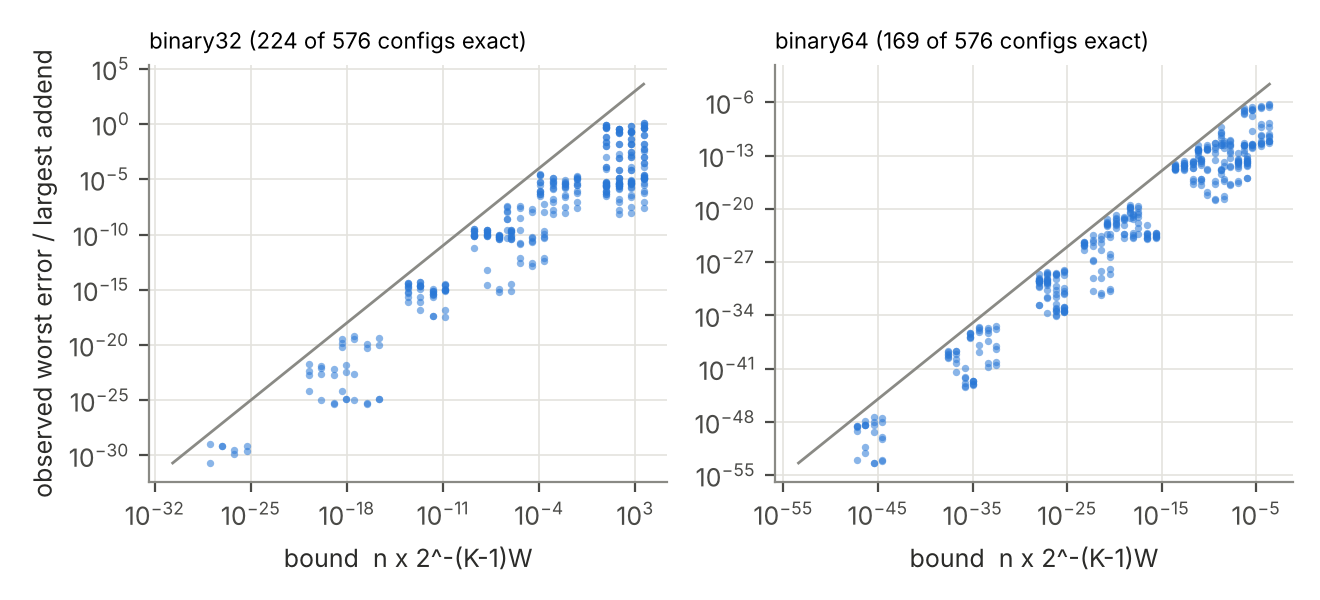
\includegraphics[width=0.95\linewidth]{./media/image1.png}
\caption{Worst observed error against the bound of Corollary 1, both
relative to the largest addend, one point per configuration. Every point
lies below the diagonal. Configurations with zero error (224 and 169 of
576) are not drawn.}\label{fig:1}
\end{figure}

\hypertarget{cost-rq4}{%
\subsection{Cost (RQ4)}\label{cost-rq4}}

CAC costs about two cell updates per contribution. Table \ref{tab:17}
gives per-contribution counts on uniform/normal data under a sequential
schedule, where no race occurs.

\begin{table}[!htbp]\centering\footnotesize\setlength{\tabcolsep}{4pt}
\caption{Per-contribution cost on uniform/normal data under a sequential schedule.}\label{tab:17}
\begin{tabularx}{\linewidth}{>{\raggedright\arraybackslash\hsize=1.980\hsize}X>{\raggedright\arraybackslash\hsize=0.848\hsize}X>{\raggedright\arraybackslash\hsize=0.778\hsize}X>{\raggedright\arraybackslash\hsize=0.990\hsize}X>{\raggedright\arraybackslash\hsize=0.636\hsize}X>{\raggedright\arraybackslash\hsize=1.061\hsize}X>{\raggedright\arraybackslash\hsize=0.707\hsize}X}
\toprule
Scheme & Format & Updates issued & Atomic operations executed & Loads & State per destination & Passes \\
\midrule
FLOAT & binary32 & 1.00 & 1.00 & 0 & 4 B & 1 \\
DOUBLE-ACC & binary32 & 1.00 & 1.00 & 0 & 8 B & 1 \\
FIXED-Q32 & binary32 & 1.00 & 1.00 & 0 & 8 B & 1 \\
WINDOW-2P & binary32 & 2.00 & 2.00 & 0 & 16 B & 2 \\
SUPERACC & binary32 & 2.86 & 1.89 & 1.00 & 76 B & 1 \\
CAC-2x32, compare-and-swap & binary32 & 1.86 & 1.86 & 1.86 & 16 B & 1 \\
CAC-2x32, native update & binary32 & 1.86 & 1.86 & 0 & 16 B & 1 \\
FLOAT64 & binary64 & 1.00 & 1.00 & 0 & 8 B & 1 \\
SUPERACC64 & binary64 & 3.01 & 2.04 & 1.00 & 532 B & 1 \\
CAC64-3x32, compare-and-swap & binary64 & 2.01 & 2.01 & 2.01 & 24 B & 1 \\
CAC64-3x32, native update & binary64 & 2.01 & 2.01 & 0 & 24 B & 1 \\
\bottomrule
\end{tabularx}
\end{table}

On binary64 gradient-like data, whose significands are full, CAC64-3x32
issues 3.00 updates per contribution and SUPERACC64 3.03. On wide-range
data the drop rule removes work: CAC-2x32 executes 1.08 atomic
operations per contribution and drops 0.57 updates after a load.

CAC and SUPERACC issue about the same number of updates. The saving of
CAC is state: 16 to 24 B against 76 B for binary32, and 24 to 32 B
against 532 B for binary64.

\textbf{Contention.} With a compare-and-swap loop, lost races cost
retries. Failure rates rise with destination skew and with the number of
warps in flight, for a floating-point compare-and-swap add and for CAC
alike.

\begin{table}[!htbp]\centering\small
\caption{Failed compare-and-swap attempts under contention.}\label{tab:18}
\begin{tabular}{llll}
\toprule
Zipf exponent & Warps in flight & \begin{tabular}[b]{@{}l@{}}FLOAT-CAS, failed\\attempts\end{tabular} & \begin{tabular}[b]{@{}l@{}}CAC-2x32, failed\\attempts\end{tabular} \\
\midrule
0 (uniform) & 64 & 7.4\% & 4.9\% \\
0 (uniform) & 512 & 35.0\% & 27.7\% \\
1 & 64 & 68.1\% & 61.4\% \\
2 & 512 & 97.8\% & 97.3\% \\
\bottomrule
\end{tabular}
\end{table}

Warp-level combining is the mitigation. At exponent 2 with 64 warps in
flight it cut the atomic operations of CAC from 3,349,152 to 201,254, a
factor of 16.6, with identical output. Combining left the output of CAC
unchanged in all 80 contention configurations; a floating-point
compare-and-swap add never matched its sequential output. The
native-update variant has no retries by construction. These rates come
from the model's random interleaving and are not hardware measurements.

\begin{figure}[!htbp]\centering
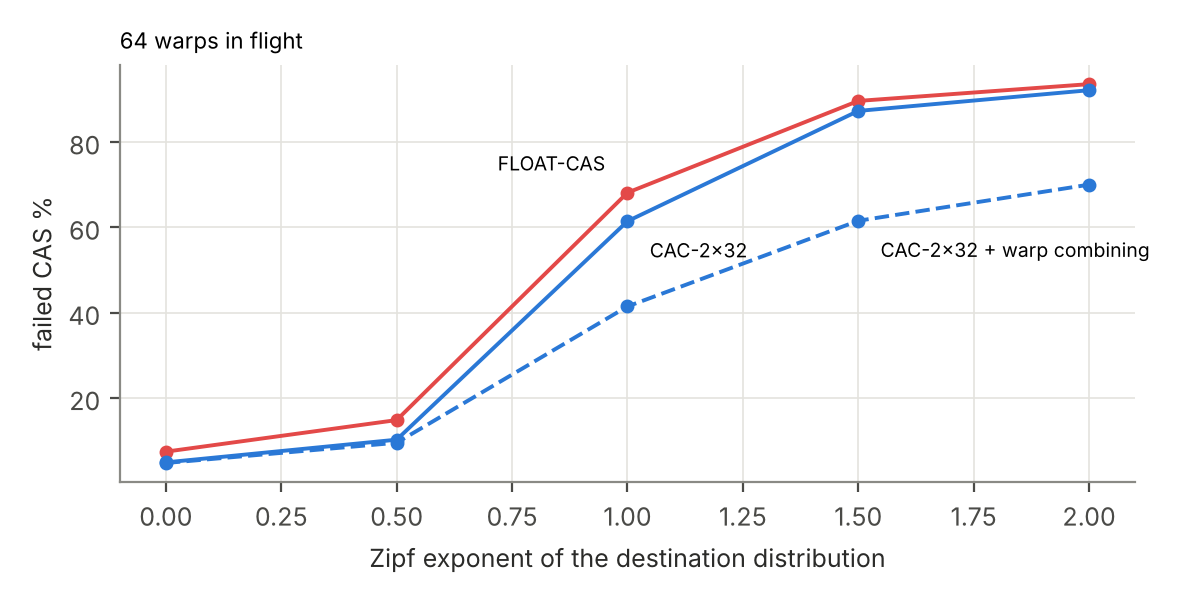
\includegraphics[width=0.62\linewidth]{./media/image2.png}
\caption{Failed compare-and-swap attempts against destination skew, 64
warps in flight, in the model.}\label{fig:2}
\end{figure}

\hypertarget{downstream-training}{%
\subsection{Downstream training}\label{downstream-training}}

The accumulation step alone made training runs differ bit for bit,
without changing what was learned. A matrix-factorisation model with
5,120 parameters was trained for 400 mini-batch SGD steps. Only the
scatter-add of gradient contributions ran on the virtual GPU, so any
difference between replicas comes from that step.

\begin{table}[!htbp]\centering\small\setlength{\tabcolsep}{4pt}
\caption{Share of parameters differing from replica 0 after 400 training steps.}\label{tab:19}
\begin{tabularx}{\linewidth}{>{\raggedright\arraybackslash\hsize=1.974\hsize}X>{\raggedright\arraybackslash\hsize=0.675\hsize}X>{\raggedright\arraybackslash\hsize=0.675\hsize}X>{\raggedright\arraybackslash\hsize=0.675\hsize}X}
\toprule
Scheme & Different schedule & Different device count & Different input order \\
\midrule
FLOAT & 84.5\% & 84.6\% & 83.6\% \\
SORT-IDX & 0 & 84.6\% & 83.6\% \\
DOUBLE-ACC, FIXED-Q32, WINDOW-2P, SUPERACC, CAC-2x32 & 0 & 0 & 0 \\
\bottomrule
\end{tabularx}
\end{table}

The entries are the share of parameters whose bits differ from replica 0
after 400 steps. With FLOAT under different schedules the share was
10.1\% after 10 steps and 63.4\% after 100. The divergence is small in
value: the largest parameter difference was \(4.8\times10^{-7}\) and the
losses differed by less than \(9\times10^{-9}\) at every step, while the
loss fell from 0.502 to 0.074. This experiment shows a reproducibility
failure. It does not show an accuracy loss.

\begin{figure}[!htbp]\centering
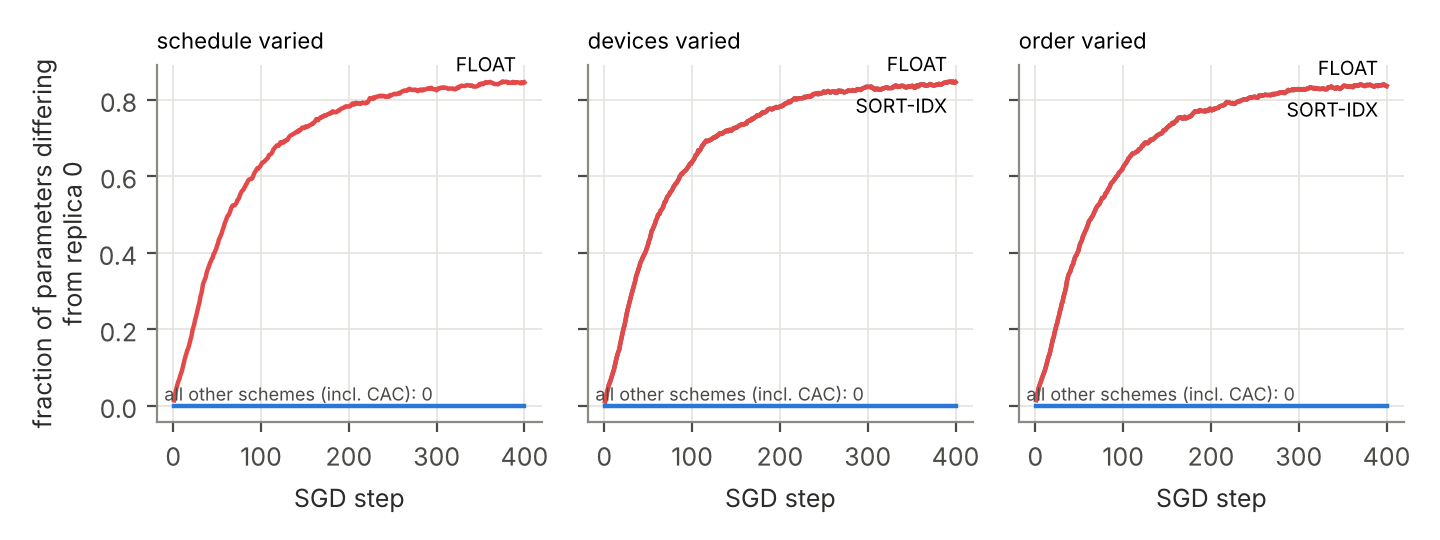
\includegraphics[width=0.95\linewidth]{./media/image3.png}
\caption{Share of parameters whose bits differ from replica 0 during
training, for each kind of variation.}\label{fig:3}
\end{figure}

\hypertarget{real-threads}{%
\subsection{Real threads}\label{real-threads}}

Under real hardware races the result was the same as in the simulator.
Each scheme ran 12 times on 4,194,304 contributions with one thread and
with two.

\begin{table}[!htbp]\centering\small
\caption{Results of the real-thread runs.}\label{tab:20}
\begin{tabular}{llll}
\toprule
Scheme & \begin{tabular}[b]{@{}l@{}}Distinct outputs\\in 12 two-thread\\runs\end{tabular} & \begin{tabular}[b]{@{}l@{}}Runs equal to the\\simulated\\sequential output\end{tabular} & \begin{tabular}[b]{@{}l@{}}Median seconds,\\two threads\end{tabular} \\
\midrule
FLOAT & 12 & 0 & 0.050 \\
FLOAT64 & 12 & 0 & 0.049 \\
DOUBLE-ACC & 1 & 12 & 0.049 \\
SUPERACC & 1 & 12 & 0.093 \\
CAC-2x32 & 1 & 12 & 0.109 \\
CAC-3x32 & 1 & 12 & 0.110 \\
SUPERACC64 & 1 & 12 & 0.123 \\
CAC64-3x32 & 1 & 12 & 0.137 \\
\bottomrule
\end{tabular}
\end{table}

On this CPU, CAC took about 2.2 times as long as a plain atomic add and
was not faster than the superaccumulator. The times describe a two-core
CPU and are not a GPU claim; they are reported so that the cost is not
hidden.

\hypertarget{how-often-a-binary64-accumulator-is-order-dependent}{%
\subsection{How often a binary64 accumulator is order
dependent}\label{how-often-a-binary64-accumulator-is-order-dependent}}

DOUBLE-ACC is order dependent in principle and almost never in practice.
A Monte Carlo experiment summed 16 binary32 addends forward and backward
in binary64 and rounded both to binary32.

\begin{table}[!htbp]\centering\small
\caption{Order dependence of a binary64 accumulator (rare-event Monte Carlo).}\label{tab:21}
\begin{tabular}{llll}
\toprule
\begin{tabular}[b]{@{}l@{}}Dynamic range of\\the addends,\\binary orders\end{tabular} & Trials & \begin{tabular}[b]{@{}l@{}}binary64\\accumulator:\\trials where the\\two orders differ\end{tabular} & \begin{tabular}[b]{@{}l@{}}Plain binary32\\accumulator:\\trials that differ\end{tabular} \\
\midrule
0 & 67,108,864 & 0 & 71.4\% \\
24 & 67,108,864 & 0 & 64.2\% \\
32 & 67,108,864 & 0 & 61.7\% \\
48 & 268,435,456 & 0 & 54.7\% \\
80 & 268,435,456 & 3 & 42.9\% \\
\bottomrule
\end{tabular}
\end{table}

The binary32 column uses 1,048,576 trials per row. For binary32 data,
DOUBLE-ACC therefore matches CAC on every standard case except overflow,
at 8 B and one atomic operation. What it lacks is a proof, and a wider
type to move to when the data is already binary64.

\hypertarget{independent-cross-check}{%
\subsection{Independent cross-check}\label{independent-cross-check}}

The Python re-derivation agreed with the C++ model on all 28,672
destinations checked, for the oracle and for two CAC configurations per
format, with no mismatch. Both implementations have the same author, so
this checks the code against the specification and not the specification
itself.

\hypertarget{discussion}{%
\section{Discussion}\label{discussion}}

The right scheme depends on the format of the data and on whether a
proof of invariance is required. CAC is the strongest option for
binary64 data and a guarantee, not an accuracy gain, for binary32 data.

\begin{table}[!htbp]\centering\small\setlength{\tabcolsep}{4pt}
\caption{Recommended scheme by situation.}\label{tab:22}
\begin{tabularx}{\linewidth}{>{\raggedright\arraybackslash\hsize=1.000\hsize}X>{\raggedright\arraybackslash\hsize=1.000\hsize}X>{\raggedright\arraybackslash\hsize=1.000\hsize}X}
\toprule
Situation & Scheme & Reason \\
\midrule
binary32 data, reproducibility wanted in practice & DOUBLE-ACC & 8 B and one atomic operation; equal to the oracle on 13 of 14 cases. Not
guaranteed, and wrong under overflow cancellation \\
binary32 data, invariance must be guaranteed & CAC-2x32 or CAC-3x32 & Proven invariant at 16 or 24 B \\
binary64 data & CAC64-3x32; CAC64-4x32 for extreme range or cancellation & No wider hardware type exists; the exact alternative needs 532 B \\
Value range known in advance and narrow & FIXED & One integer atomic; exact inside the window \\
Contributions cheap to generate twice & WINDOW-2P & Same accuracy as CAC-2x32 with plain integer atomics and no retry loop \\
Sums that cancel far below their largest addend & SUPERACC & The only scheme correct on all 14 cases \\
\bottomrule
\end{tabularx}
\end{table}

\hypertarget{what-the-results-establish}{%
\subsection{What the results
establish}\label{what-the-results-establish}}

\begin{itemize}
\item
  \textbf{RQ1.} The irreproducibility of floating-point scatter-add can
  be regenerated exactly from a seed: 32 outputs from 32 schedules in
  all 28 cases.
\item
  \textbf{RQ2.} A bounded-state, single-pass, order-invariant mechanism
  exists. Its invariance is proven and was never violated: 420 gates,
  1,152 sensitivity configurations, 80 contention configurations and 72
  real-thread runs of CAC.
\item
  \textbf{RQ3.} Outside the overflow case, CAC with enough cells missed
  at most five of 53,248 destinations, and the error bound held
  everywhere.
\item
  \textbf{RQ4.} The price is about two to three cell updates per
  contribution and 16 to 32 B per destination, against 76 to 532 B for
  an exact accumulator.
\end{itemize}

\hypertarget{what-the-results-do-not-establish}{%
\subsection{What the results do not
establish}\label{what-the-results-do-not-establish}}

\begin{itemize}
\item
  \textbf{Speed.} No physical GPU was used. The only timing, on a CPU,
  shows CAC at about 2.2 times the cost of a plain atomic add.
\item
  \textbf{An accuracy advantage for binary32.} DOUBLE-ACC was as
  accurate as CAC on every standard case where either worked.
\item
  \textbf{Harm from irreproducibility.} The training experiment shows
  different bits and the same loss.
\item
  \textbf{Safety under deep cancellation.} A result far below its
  largest addend is lost, without any signal.
\item
  \textbf{Novelty beyond the survey.} The claim of Section 3.1 covers
  the cited literature only.
\end{itemize}

\hypertarget{limitations-and-threats-to-validity}{%
\section{Limitations and threats to
validity}\label{limitations-and-threats-to-validity}}

The main limitation is that CAC has not run on a GPU. The others bound
what the mechanism itself can do.

\hypertarget{limits-of-the-mechanism}{%
\subsection{Limits of the mechanism}\label{limits-of-the-mechanism}}

\begin{itemize}
\item
  \textbf{Accuracy is relative to the largest addend.} When a sum
  cancels below the window, the result is lost and nothing reports it.
  The read-out knows the top bin, so it could flag a result that is
  small against the bound of Theorem 3; this is not implemented or
  evaluated.
\item
  \textbf{binary64 needs at least three cells.} With K = 2 the window is
  narrower than the significand.
\item
  \textbf{Capacity is finite.} A destination can absorb \(2^{55−W}\)
  addends before a cell value wraps. The counters for zeros and
  infinities are 28 bits wide, so \(2^{28}\) same-signed zeros or
  infinities at one destination would be misread.
\item
  \textbf{The state is not a floating-point array.} A destination buffer
  becomes K 64-bit words, and a read-out pass is needed before the
  values can be used. In-place accumulation into an existing tensor does
  not apply directly.
\item
  \textbf{The result differs from every floating-point order.} CAC
  returns the rounding of a near-exact sum. Code that expects the value
  of one particular sequential order will see a different, usually more
  accurate, value.
\item
  \textbf{Compare-and-swap retries.} Without a native update, heavy skew
  causes many retries. Warp combining reduced them in the model; its
  cost on hardware is unknown.
\end{itemize}

\hypertarget{threats-to-validity}{%
\subsection{Threats to validity}\label{threats-to-validity}}

\begin{itemize}
\item
  \textbf{Simulator, not hardware.} The model checks functional
  behaviour under legal interleavings. It does not model memory
  hierarchy, atomic-unit throughput or real scheduling, and failure
  rates under its random scheduler are indicative only.
\item
  \textbf{Synthetic workloads.} The 14 cases are constructed to span
  patterns and ranges. They are not traces of real applications.
\item
  \textbf{A small training experiment.} One model, 5,120 parameters, 400
  steps. It shows that bits diverge and says nothing about larger models
  or chaotic training regimes.
\item
  \textbf{One author for model and cross-check.} The Python cross-check
  shares the author's reading of the specification. An independent
  implementation would be stronger evidence.
\item
  \textbf{Baseline fidelity.} The baselines are our models of published
  ideas, not the original codes. SUPERACC is a carry-save variant and is
  larger than the design in {[}9{]}. FIXED uses one scale per format.
\item
  \textbf{Survey coverage.} The novelty claim rests on a literature
  search that may have missed work, especially in hardware patents and
  vendor libraries.
\item
  \textbf{Reference metadata.} Bibliographic details were collected from
  publisher and archive pages and should be re-checked before
  submission.
\end{itemize}

\hypertarget{reproducibility}{%
\section{Reproducibility}\label{reproducibility}}

Every number in this paper can be regenerated with three commands on a
machine with a C++17 compiler and Python 3 with matplotlib. The full run
takes under five minutes on two cores.

\begin{lstlisting}
make          # build ./cac (g++ or clang++)
make test     # 55 tests
make results  # experiments, cross-check,
              # tables and figures
\end{lstlisting}

\begin{table}[!htbp]\centering\small\setlength{\tabcolsep}{4pt}
\caption{Reproduction steps and expected outputs.}\label{tab:23}
\begin{tabularx}{\linewidth}{>{\raggedright\arraybackslash\hsize=0.930\hsize}X>{\raggedright\arraybackslash\hsize=1.070\hsize}X}
\toprule
Step & Expected output \\
\midrule
make test & 55/55 registered tests passed \\
Sensitivity (inside make results) & 576 evaluations, 0 bound violations, once per format \\
Cross-check (inside make results) & 28672 destination checks, 0 mismatching columns \\
Tables and figures & results/tables.md and results/figures/ \\
\bottomrule
\end{tabularx}
\end{table}

Three rules keep the results bit-identical across machines.

\begin{itemize}
\item
  \textbf{Integer randomness.} All seeds feed an integer xoshiro256**
  generator; normal variates are sums of uniform draws.
\item
  \textbf{No contraction.} The build passes -ffp-contract=off, so no
  fused multiply-add changes a workload.
\item
  \textbf{Frozen digests.} The tests compare a hash of every standard
  workload with a stored value and fail if a platform generates
  different data.
\end{itemize}

One output is not expected to repeat. The real-thread experiment depends
on the machine and the moment, in its timings and in the outputs of
FLOAT; only the invariant schemes repeat there. The Monte Carlo counts
of Section 8.8 do repeat, because each random stream has a fixed seed
whatever the number of threads.

The artifact contains the simulator source, the test suite, the
experiment driver, both scripts and the raw CSV files from which this
paper's tables were produced.

\hypertarget{conclusion-and-future-work}{%
\section{Conclusion and future work}\label{conclusion-and-future-work}}

Floating-point scatter-add can be made independent of execution order
with two to four 64-bit words per destination, in one pass, with no
knowledge of the value range. The mechanism is a commutative monoid on
tagged cells, and its order invariance is a theorem that the reference
model never contradicted.

The evidence also marks where CAC should not be used. It loses results
that cancel far below their largest addend, it needs three cells for
binary64, and for binary32 data a binary64 accumulator is cheaper and
was as accurate in practice.

Four steps follow.

\begin{enumerate}
\def\labelenumi{\arabic{enumi}.}
\item
  \textbf{A GPU implementation.} A CUDA kernel using 64-bit atomicCAS,
  measured against atomicAdd on a consumer GPU, would replace the cost
  model with timings.
\item
  \textbf{A cancellation flag.} The read-out can compare the result with
  the bound of Theorem 3 and report results that are not trustworthy.
\item
  \textbf{Adaptive width.} Destinations could start with two cells and
  grow only where the flag fires.
\item
  \textbf{Framework integration.} A deterministic index\_add and
  scatter\_add built on CAC would test the idea on real training
  workloads.
\end{enumerate}

\begin{thebibliography}{99}
\bibitem{ref1} D. Goldberg. What every computer scientist should know about
floating-point arithmetic. \emph{ACM Computing Surveys} 23(1), 1991.

\bibitem{ref2} N. J. Higham. The accuracy of floating point summation. \emph{SIAM
Journal on Scientific Computing} 14(4), 1993.

\bibitem{ref3} S. Shanmugavelu, M. Taillefumier, C. Culver, O. Hernandez, M. Coletti,
A. Sedova. \href{https://arxiv.org/pdf/2408.05148}{Impacts of
floating-point non-associativity on reproducibility for HPC and deep
learning applications}. SC24 Workshops, 2024. arXiv:2408.05148.

\bibitem{ref4} PyTorch documentation. Reproducibility notes and
torch.use\_deterministic\_algorithms. Consulted November 2026.

\bibitem{ref5} N. Cankaya. \href{https://arxiv.org/html/2606.00279v2}{Bit-exact AI
inference verification without performance tradeoffs}. arXiv:2606.00279,
2026.

\bibitem{ref6} H. Jooybar, W. W. L. Fung, M. O'Connor, J. Devietti, T. M. Aamodt.
GPUDet: a deterministic GPU architecture. ASPLOS 2013.

\bibitem{ref7} Y. H. Chou, C. Ng, S. Cattell, J. Intan, M. D. Sinclair, J. Devietti, T.
G. Rogers, T. M. Aamodt. Deterministic atomic buffering. MICRO 2020,
pp.~981--995. DOI 10.1109/MICRO50266.2020.00083.

\bibitem{ref8} S. Le Grand, A. W. Götz, R. C. Walker. SPFP: speed without compromise
--- a mixed precision model for GPU accelerated molecular dynamics
simulations. \emph{Computer Physics Communications} 184(2), 2013.

\bibitem{ref9} D. Defour, C. Collange.
\href{https://annals-csis.org/proceedings/2015/drp/86.html}{Reproducible
floating-point atomic addition in data-parallel environment}. FedCSIS
2015, ACSIS vol.~5, pp.~721--728. DOI 10.15439/2015F86.

\bibitem{ref10} C. Collange, D. Defour, S. Graillat, R. Iakymchuk.
\href{https://hal-lirmm.ccsd.cnrs.fr/lirmm-01206348/document}{Numerical
reproducibility for the parallel reduction on multi- and many-core
architectures}. \emph{Parallel Computing} 49, pp.~83--97, 2015. DOI
10.1016/j.parco.2015.09.001.

\bibitem{ref11} J. Demmel, H. D. Nguyen. Fast reproducible floating-point summation.
21st IEEE Symposium on Computer Arithmetic, pp.~163--172, 2013.

\bibitem{ref12} P. Ahrens, J. Demmel, H. D. Nguyen. Algorithms for efficient
reproducible floating point summation. \emph{ACM Transactions on
Mathematical Software} 46(3), 2020.

\bibitem{ref13} I. Müller, A. Arteaga, T. Hoefler, G. Alonso. Reproducible
floating-point aggregation in RDBMSs. ICDE 2018. arXiv:1802.09883.

\bibitem{ref14} R. M. Neal. Fast exact summation using small and large
superaccumulators. arXiv:1505.05571, 2015.

\bibitem{ref15} U. Kulisch, W. L. Miranker. \emph{Computer Arithmetic in Theory and
Practice}. Academic Press, 1981.

\bibitem{ref16} M. Shapiro, N. Preguiça, C. Baquero, M. Zawirski. Conflict-free
replicated data types. SSS 2011.

\bibitem{ref17} IEEE Standard for Floating-Point Arithmetic, IEEE Std 754-2019.

\bibitem{ref18} pyscf/gpu4pyscf, GitHub issue \#1007: Run-to-run non-determinism from
floating-point atomics. Opened 31 October 2026.
https://github.com/pyscf/gpu4pyscf/issues/1007

\bibitem{ref19} openvinotoolkit/openvino, GitHub pull request \#37458: {[}GPU{]} Add a
local-memory-staged fast path for dense SUM ScatterElementsUpdate.
https://github.com/openvinotoolkit/openvino/pull/37458
\end{thebibliography}

\end{document}
